% Vector-preserving 2x2 composite of the four key-lifecycle phase figures.
% Built at 390pt total width (= 12pt single-column text width), so panel
% labels render at true 9pt. Rows use equal image heights; row heights
% differ because the aspect mixes (portrait panel (d) sets row 2's height).
\documentclass[border=4pt]{standalone}
\usepackage{graphicx}
\begin{document}
\begin{minipage}{390pt}\centering
% Row 1: (a) 1875x1416  (b) 2420x2460 — equal height 165.5pt
\begin{minipage}[t]{219.2pt}\centering
  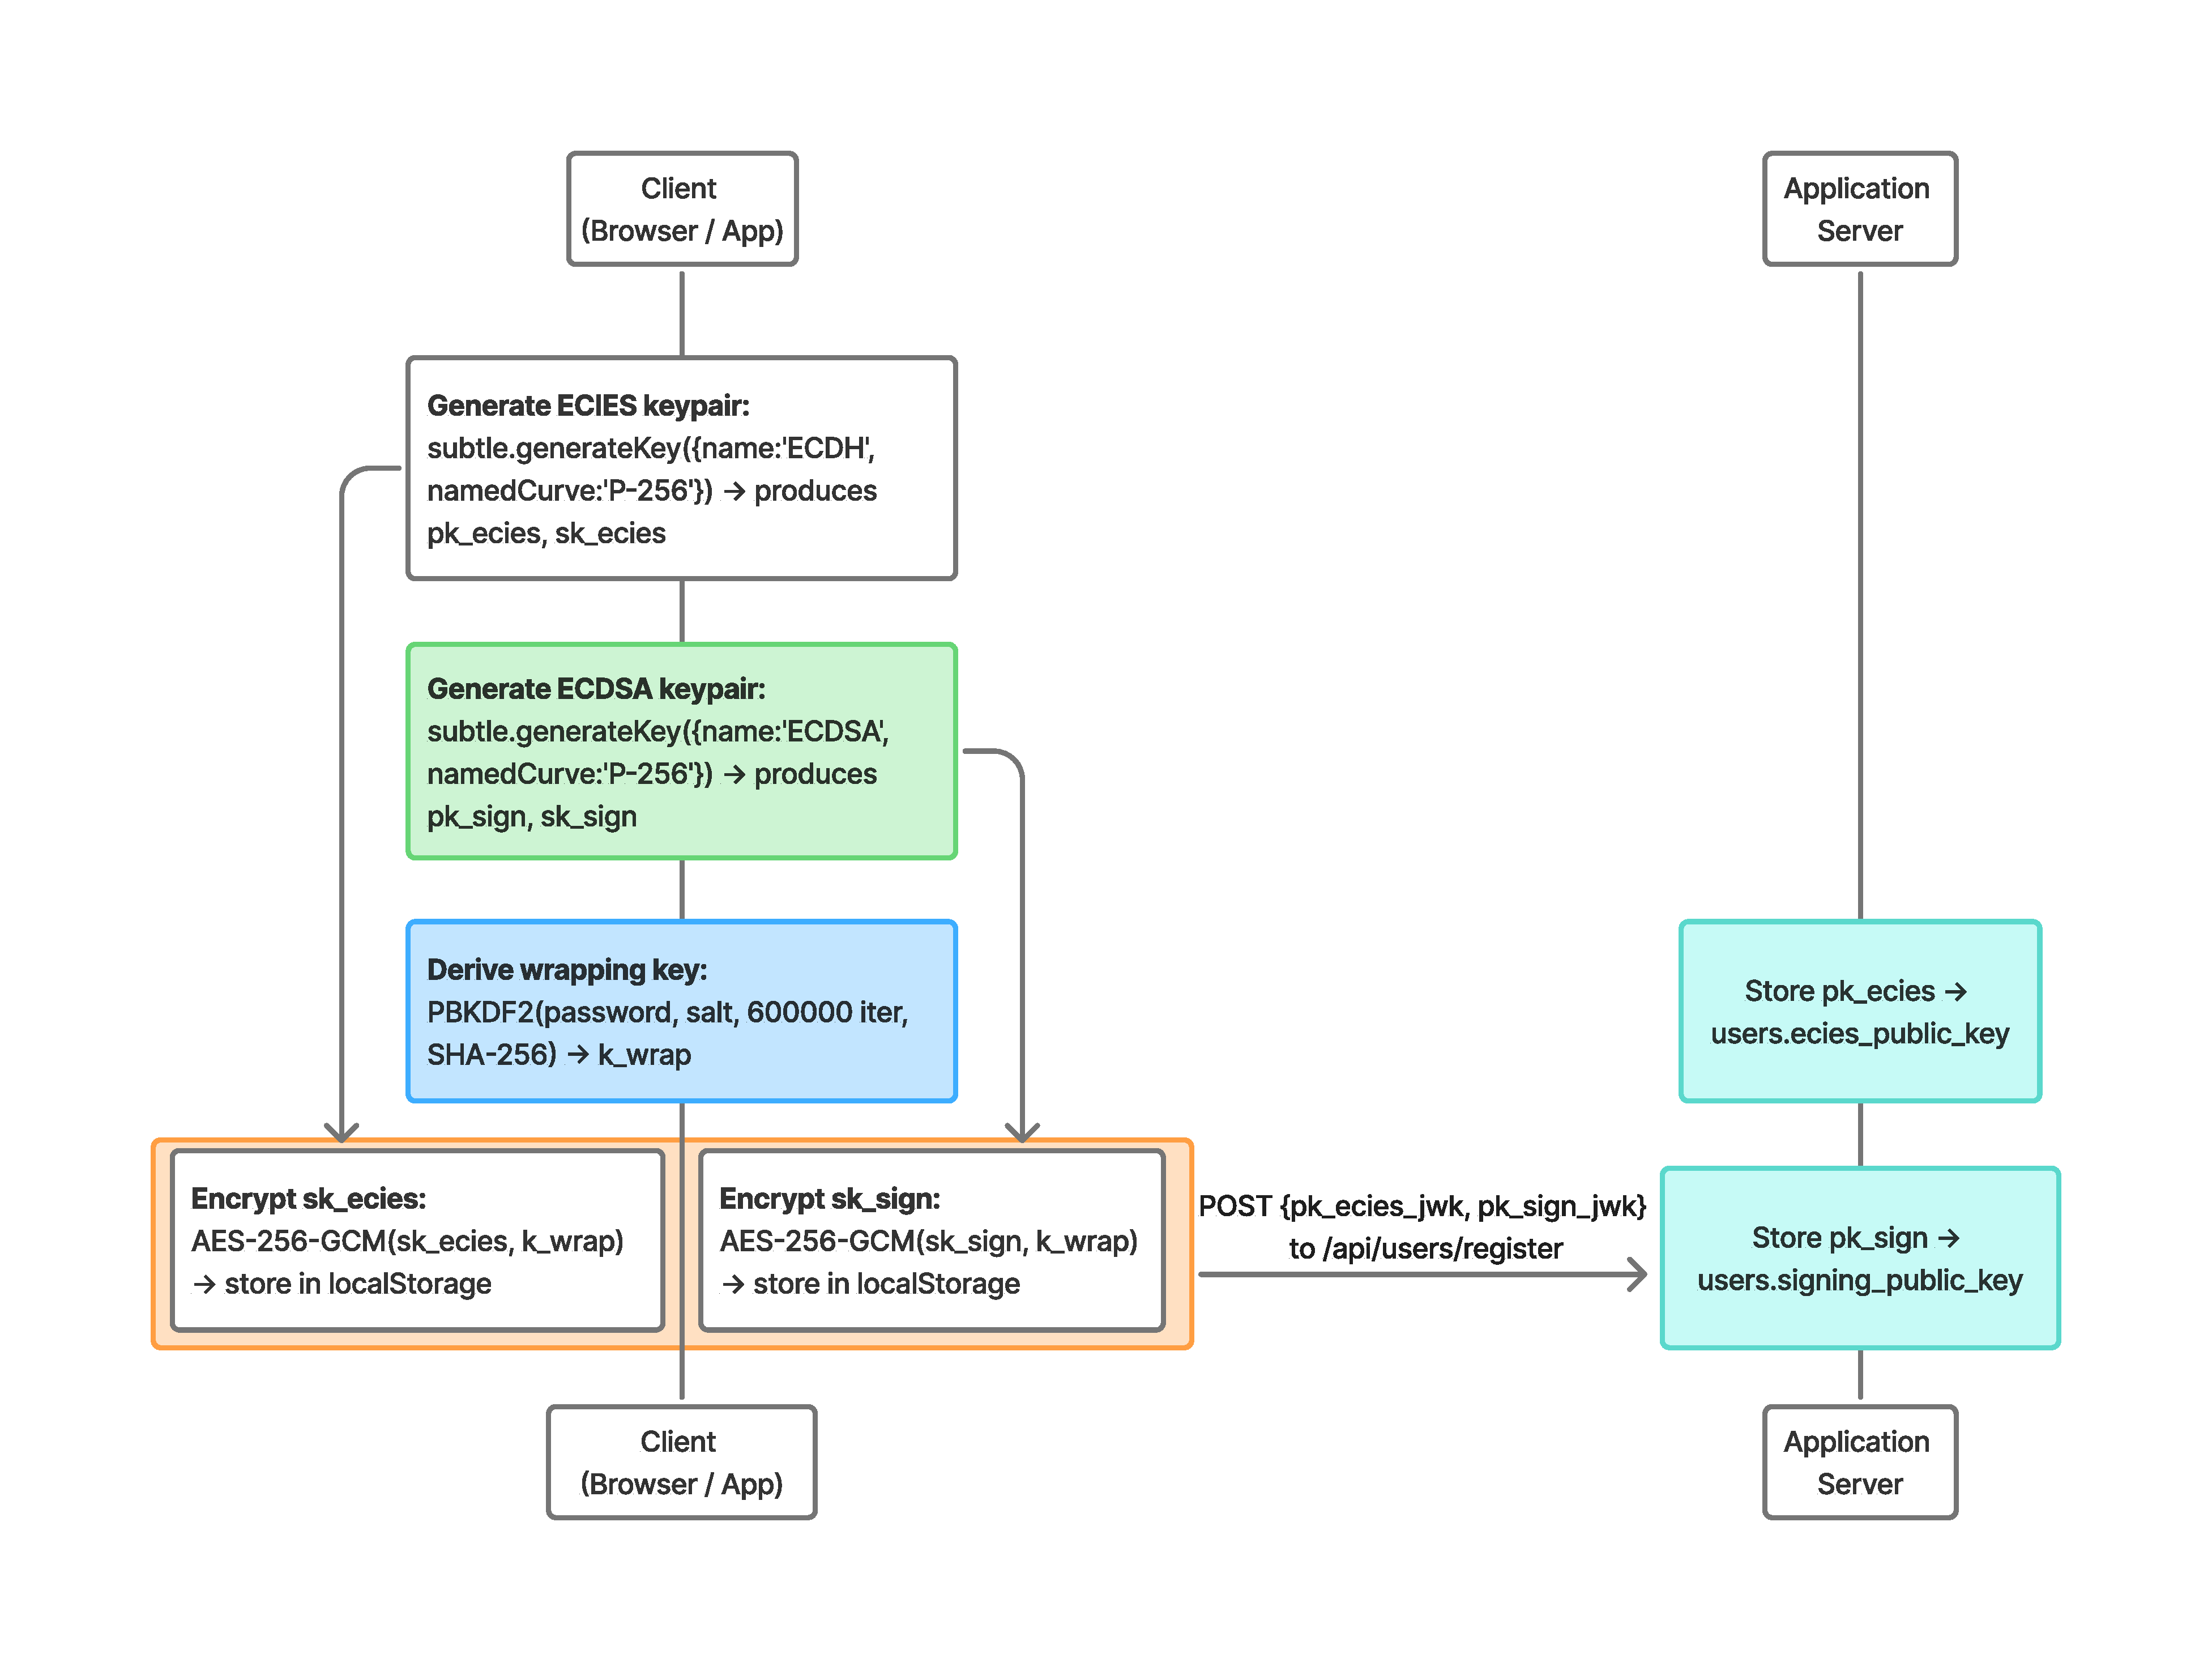
\includegraphics[height=165.5pt]{key_gen_and_storage.pdf}\\[3pt]
  {\fontsize{9}{11}\selectfont (a) Phase 1: key generation and storage}
\end{minipage}\hfill
\begin{minipage}[t]{162.8pt}\centering
  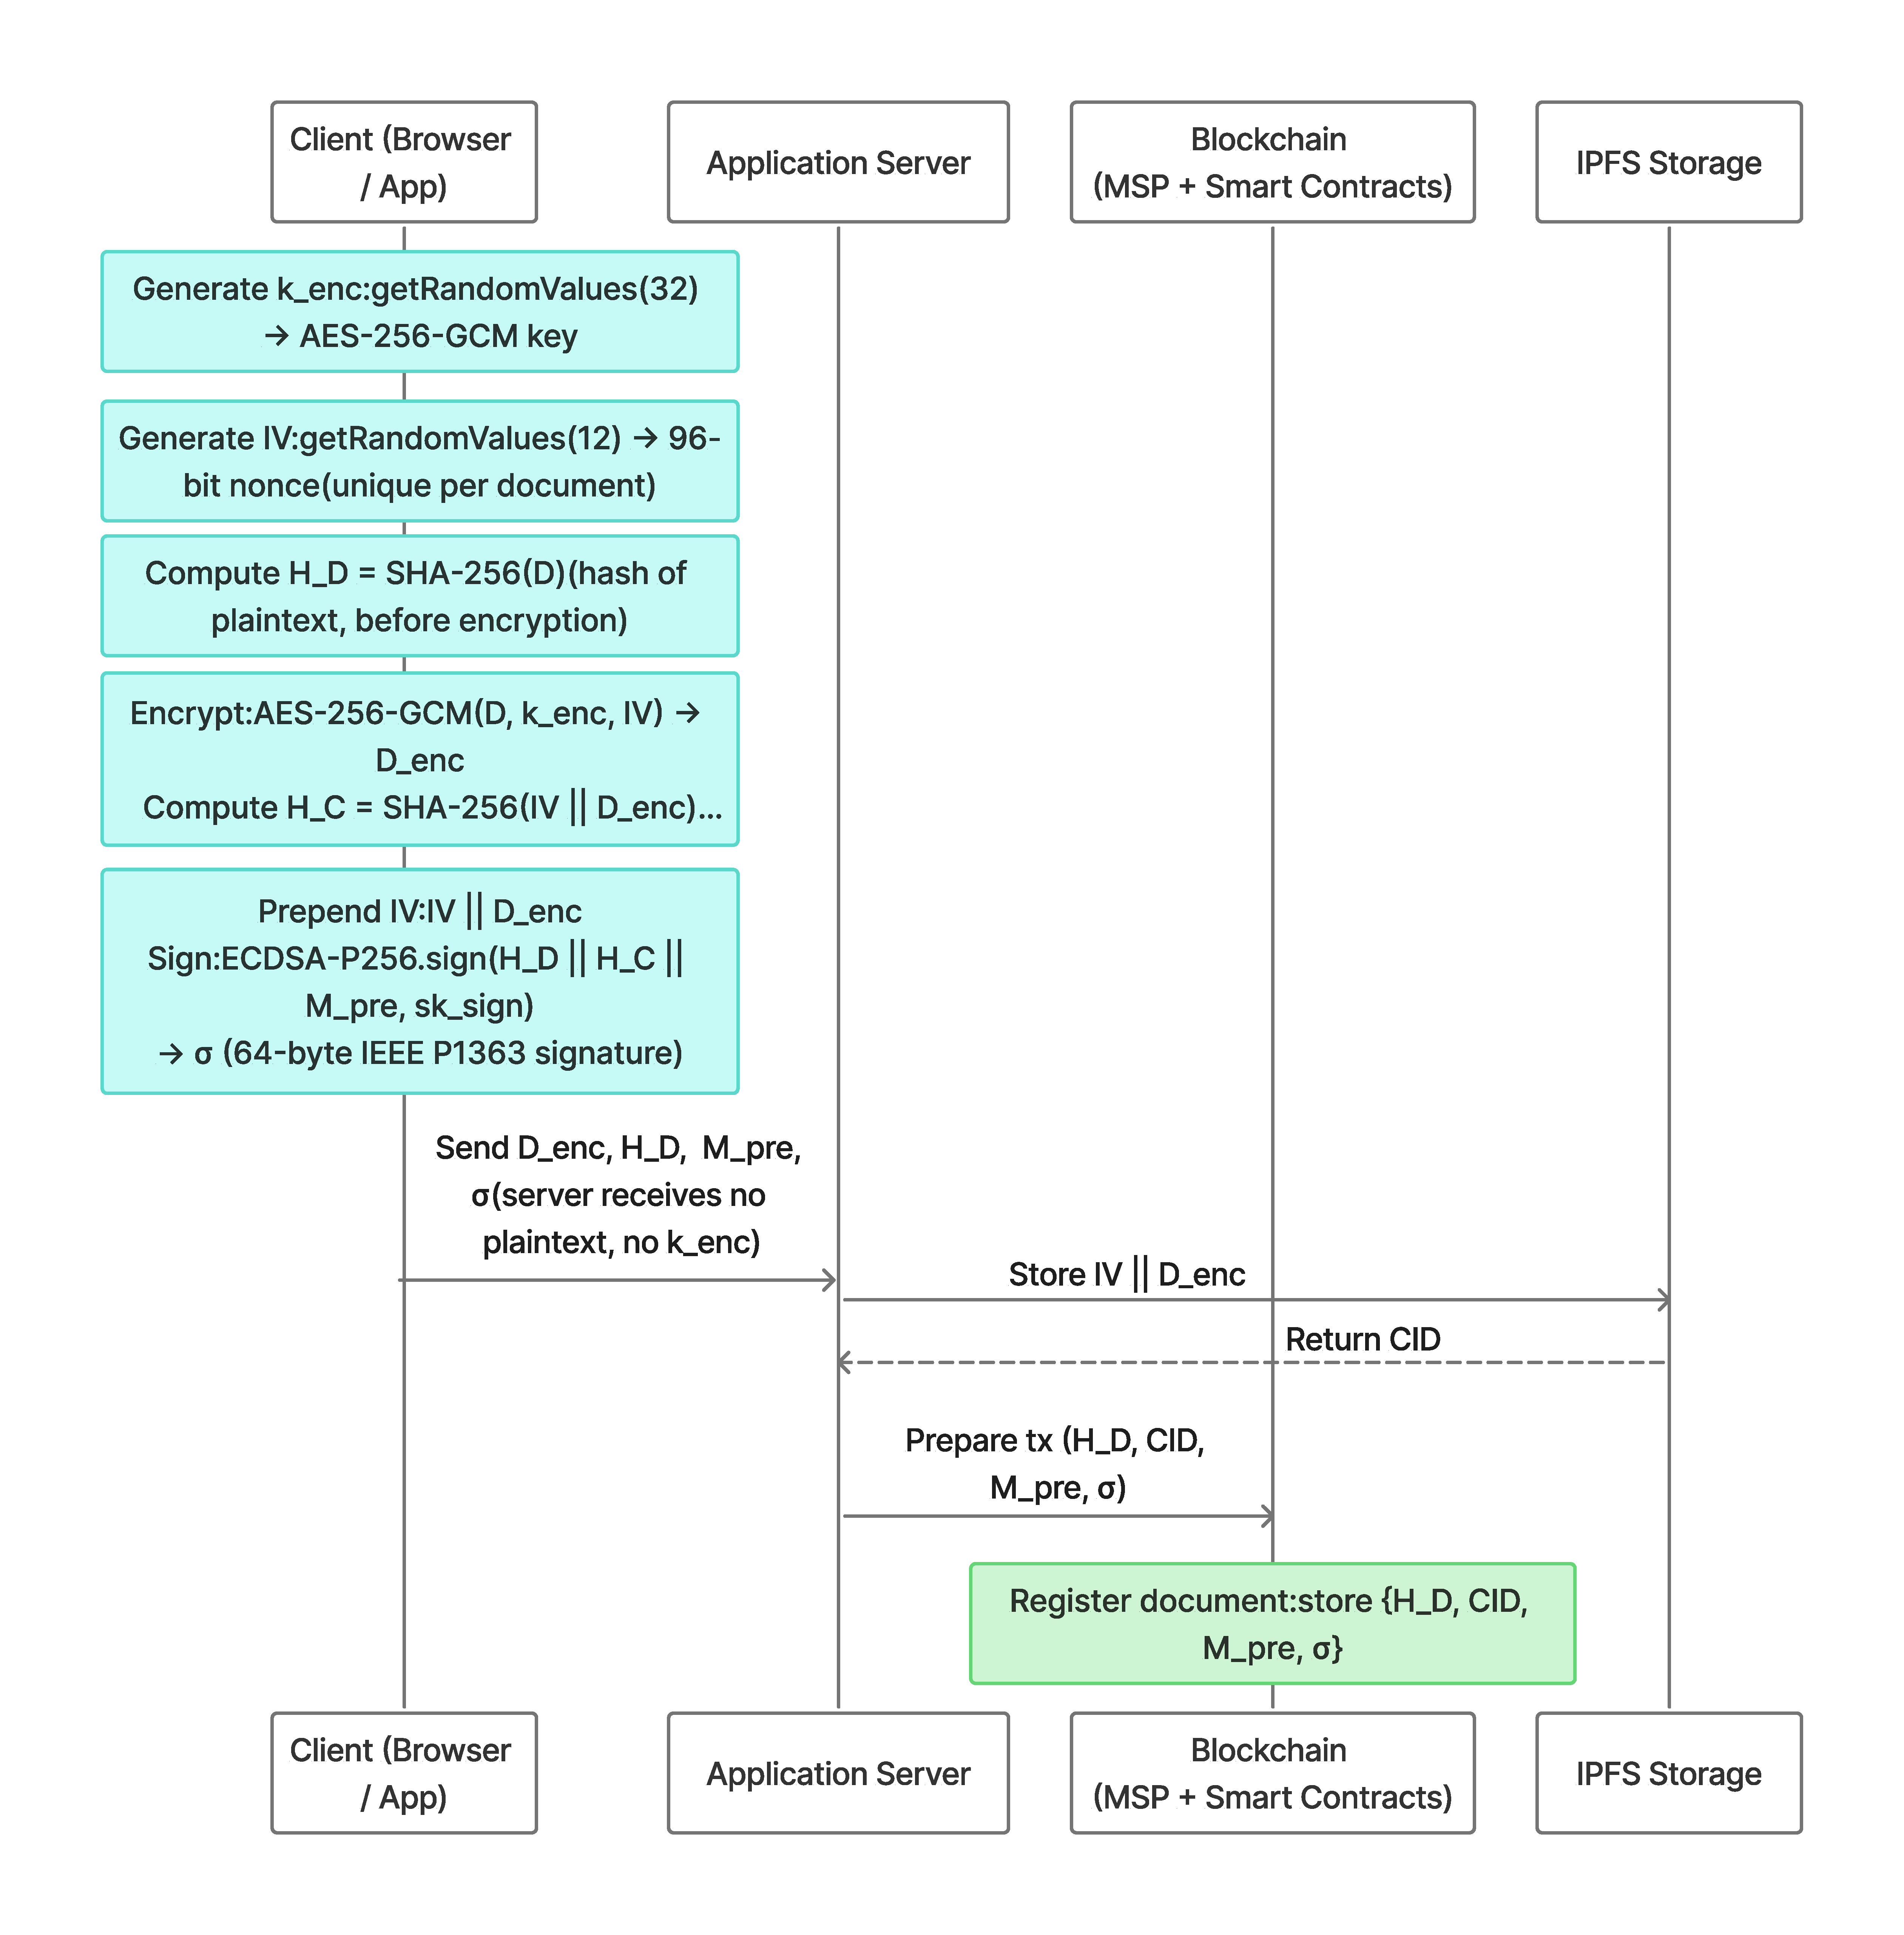
\includegraphics[height=165.5pt]{document_encryption.pdf}\\[3pt]
  {\fontsize{9}{11}\selectfont (b) Phase 2: document encryption and registration}
\end{minipage}
\par\vspace{10pt}
% Row 2: (c) 2534x1920  (d) 2296x3012.55 (portrait) — equal height 183.5pt
\begin{minipage}[t]{242.2pt}\centering
  
\includegraphics[height=183.5pt]{access_grant.pdf}\\[3pt]
  {\fontsize{9}{11}\selectfont (c) Phase 3: access grant and key wrapping}
\end{minipage}\hfill
\begin{minipage}[t]{139.8pt}\centering
  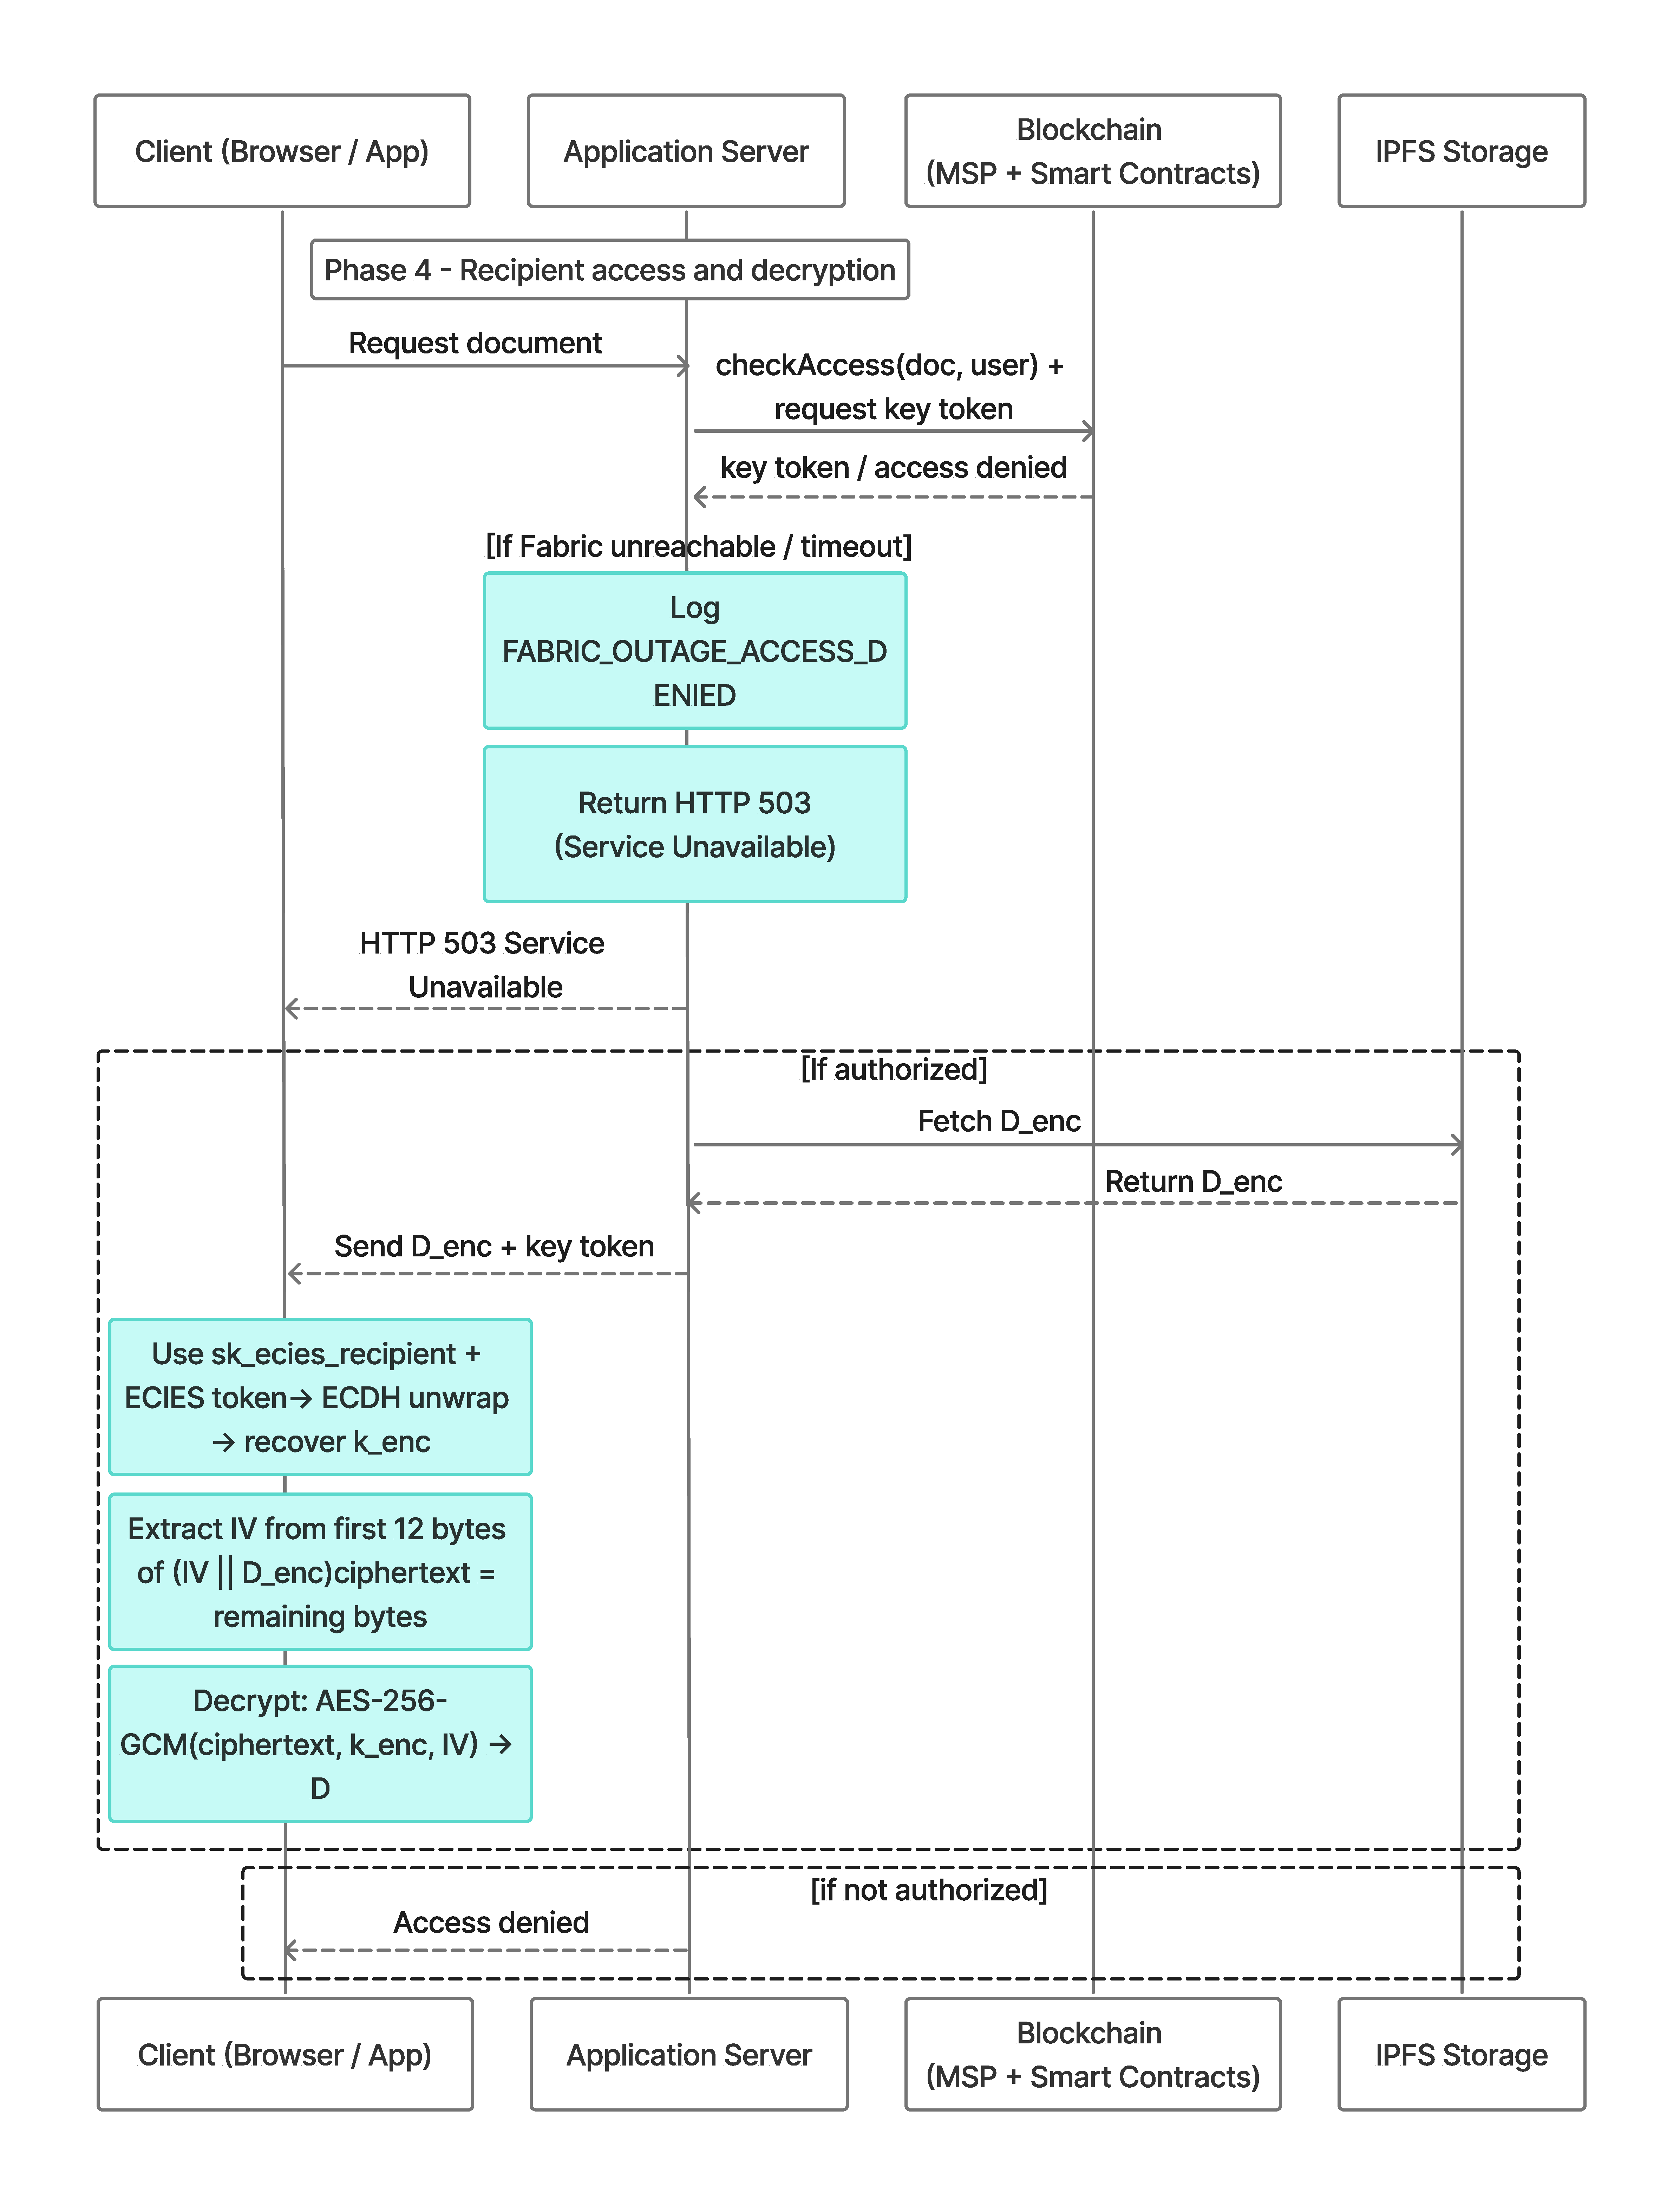
\includegraphics[height=183.5pt]{access_and_decryption.pdf}\\[3pt]
  {\fontsize{9}{11}\selectfont (d) Phase 4: access and decryption}
\end{minipage}
\end{minipage}
\end{document}
